\section{Calculus}

\begin{definition}[Adiabatic]
    adiabatic wall between two thermodynamic systems does not allow heat or
    matter to pass across it. 

\end{definition}

\begin{definition}[A priori estimate]
    An estimate for a size of a solution or it's deriviates of a PDE.\
    The estimate is made before the solution is known to exists.

\end{definition}

\begin{definition}[Affine]
    $ 
    f(x_{1}, x_{2}, \dots, x_{n}) = 
    a_{1}x_{1}, a_{2}x_{2}, \dots a_{n}x_{n}
    $
\end{definition}

\begin{definition}[Analytic function]
    A function given by~\nameref{convergence}~\nameref{powerseries}.
    
    Any polynomial, exponential and trigonometric function is analytic.
    Functions that are not differentiable at given points are not analytic.

\end{definition}

\begin{definition}[arcsin]
    \begin{align*}
        \sin{y} &= x \\
        \arcsin{x} &= \sin^{-1}{x} = y
    \end{align*}

    Properties:
    \begin{itemize}
        \item $\arcsin{x} = \frac{\pi}{2} - \arccos{x} = 90º - \arccos{x}$
        \item $\cos{(\arcsin{x}} = \sin{(\arccos{x})} = \sqrt{1-x^{2}}{}$
        \item $ x = -1 \rightarrow \arcsin{x} = -1\times\frac{\pi}{2}$
        \item $ x = 1 \rightarrow \arcsin{x} = \frac{\pi}{2}$
        \item $ x = 0 \rightarrow \arcsin{x} = 0$
    \end{itemize}
\end{definition}

\begin{definition}[arccos]\label{arccos}
    Properties:
    \begin{itemize}
        \item $ x = -1 \rightarrow \arccos{x} = \pi$
        \item $ x = 1 \rightarrow \arccos{x} = 0$
        \item $ x = 0 \rightarrow \arccos{x} = \frac{\pi}{2}$
    \end{itemize}
\end{definition}

\begin{definition}[Arc length]
    Length of a curve when straightened out.
\end{definition}
\begin{definition}[arccos]
    While cosine shows the relation between lengths in a triangle, 
    arccos gives the angle.
\end{definition}

\begin{definition}[Arithmetic-geometric mean inequality]\label{arigeo}
    $
    \newline {(\prod\limits_{i = 1}^{k} a_{i})}^{1/k}
    \leq {1 \over k} \sum\limits_{i = 1}^{k} a_{i}
    $
\end{definition}

\begin{definition}[Azimuth]
     is an angular measurement in a spherical coordinate system. The vector
     from an observer (origin) to a point of interest is projected
     perpendicularly onto a reference plane; the angle between the projected
     vector and a reference vector on the reference plane is called the
     azimuth.

     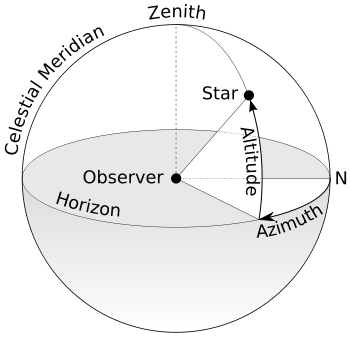
\includegraphics[scale=0.3]{azimuth.png}

\end{definition}

\begin{definition}[Bijection]
    \begin{align}
        S,R \text{\ are sets} \\
        \forall{i \in S}, \exists!{f(i) \in R} \wedge \\
        \forall{i \in R}, \exists!{f(i) \in S} \\
    \end{align}
\end{definition}

\begin{definition}[Boundary value problem]
    A differential equation with additional restrains. A solution to a boundary
    value problem is a solution to the differential equation which also
    satisfies the boundary conditions.
    
\end{definition}


\begin{definition}[Cauchy sequence]
    a sequence whose elements become arbitrarily close to each other as the
    sequence progresses.
    Think of \textit{two} curves that approximate each other.

\end{definition}

\begin{definition}[Cardinal number, ]
    The size of a set.
\end{definition}

\begin{definition}[Convergence]\label{convergence}
    A series is convergent is the sum of it's elements approaches a given 
    number.
\end{definition}

\begin{definition}[Convolution]
    Dictionary: a coil or twist, especially one of many.\newline
    Informal: an expression of how a shape from one function is modified by 
        the other.

    Can also be used to smoothen a discontinous a function (making it continous 
    on the given range). We need to normalize our g(x - $\tau$) so that we do
    not continously increase the f(x)
\end{definition}

\begin{definition}[Continuous]
In mathematics, a continuous function is a function for which
"small" changes in the input result in "small" changes in the output.

As an example, consider the function h(t), which describes the height of a
growing flower at time t. This function is continuous. By contrast, if M(t)
denotes the amount of money in a bank account at time t, then the function
jumps whenever money is deposited or withdrawn, so the function M(t) is
discontinuous.

\end{definition}

\begin{definition}[Continuous variables]
    There are three types of continuous variables:
    \begin{center}
    \begin{description}
        \item[Nominal] Categorized within groups: box 1, 2, 3 or 4.
        \item[Dichotomous] Boolean, yes or no.
        \item[Ordinal] A nominal variable, just that different groups give
            different values. E.g.\ to like something on a scale of 1 to 10
            gives you a ordinal range
    \end{description}
\end{center}
\end{definition}

\begin{definition}[Conjugate]
     is a binomial formed by negating the second term of a binomial. The
     conjugate of $x + y$ is $x − y$.

\end{definition}

\begin{definition}[Concave]
    Let $f$ be a function defined on the interval $[x_{1}, x_{2}]$.
    This function is concave according to the definition if, for every pair of
    numbers a and b with $x_{1} \leq a \leq x_{2}$ and $x_{1} \leq b \leq
    x_{2}$, the line segment from $(a,  f (a))$ to $(b,  f (b))$
    lies on or below the function.

    \begin{itemize}
        \item The sine function is concave on the interval $[0, \pi]$
        \item Concave if every line segment joining two point is never above
              the graph 
        \item Concave functions has $f\prime\prime(x) \leq 0$ in a given
              interval 
    \end{itemize}
\end{definition}

\begin{definition}[Congruence]
    Similar shape and growth, just different scalar / rotation.
\end{definition}


\begin{definition}[Damping]
    is an influence within or upon an oscillatory system that has the effect of
    reducing, restricting or preventing its oscillations. 
    Underdamped systems will start bouncy and then stop.

\end{definition}

\begin{definition}[Differential operator]
    An operator to do differentiation. This is mainly to abstract
    differenentiation.

\end{definition}

\begin{definition}[Discrete Fourier Transform]\label{dft}
    converts a finite list of equally spaced samples of a function into the
    list of coefficients of a finite combination of complex sinusoids, ordered
    by their frequencies, that has those same sample values.

\end{definition}

\begin{definition}[Discrete Laplace transform]
    An integral transfrom, which in 2d uses the kernel
    % \begin{bmatrix}   
    %     0 & 1 & 0 \\  
    %     1 & -4 & 1 \\ 
    %     0 & 1 & 0     
    % \end{bmatrix}     
\end{definition}

\begin{definition}[Discrete Sine Transform]
    Similar to~\nameref{dft}, but uses only a real matrix.

\end{definition}

\begin{definition}[Discretization]
    concerns the process of transferring
    continuous models and equations into discrete counterparts. 
    AKA\ smoothening curves to avoid jumps.

\end{definition}

\begin{definition}[Displacement]
    The shortest distance from source $s$ to $t$ (like air-distance).

\end{definition}

\begin{definition}[Divergence]\label{divergence}
    measures the magnitude of a~\nameref{vectorfield}'s source or sink at a
    given point, in terms of a signed scalar.

    E.g.\ air can be thought of to have a point $s \text{ and } t$, where they
    push out hot and cool air, respectively. From these points, you can create
    a~\nameref{vectorfield} that shows how air spreads from $s \text{ and }
    t$. The divergence measures the collected value from each of 
    these~\nameref{vectorfield}s.

    The operator for divergence is \verb|{div}|, represented by nabla.

    Given vector field $F = Ui, Vj, Wk$:
    \begin{align}
            div \textbf{F} = \nabla \cdot F = 
            \frac{\partial{U}}{\partial{x}}+
            \frac{\partial{V}}{\partial{y}} +
            \frac{\partial{W}}{\partial{z}}
    \end{align}

\end{definition}

\begin{definition}[Elementary function]
    In mathematics, an elementary function is a function of one variable built
    from a finite number of exponentials, logarithms, constants, and $nth$ roots
    through composition and combinations using the four elementary operations
    $(+ – × ÷)$.

\end{definition}

\begin{definition}[Expansion function]
    A function, with a series, to express a function. The series will in
    most cases be an approximation to the original function.
    Signal functions are often modeled using expansion functions.
\end{definition}

\begin{definition}[Eulers formula]
    $e^{ix} = \cos{x} + i\sin{x}$
\end{definition}

\begin{definition}[Explicit methods]\label{explicitmethod}
    In numerical analysis, an explicit method calculates the state of the system
    using only earlier history. See also~\nameref{implicitmethod}.
\end{definition}


\begin{definition}[Extreme point]
    A point furthest away from something.
\end{definition}

\begin{definition}[Field]
    A physcial quantity that has a value for each point in space and time.
\end{definition}

\begin{definition}[Finite difference]
    The difference in a function for $f(x + a) - f(x + b)$.

    There are three types:
    \begin{description}
        \item[Forward] is of the form $\bigtriangleup{f}(x) = f(x + h) - f(x)$
        \item[Backward] is of the form $\nabla{f}(x) = f(x) - f(x - h)$
        \item[Centered] is of the form $\delta{f}(x) = f(x + \frac{1}{2}h) - f(x - \frac{1}{2}h)$
    \end{description}
\end{definition}

\begin{definition}[Finite element method]
    (FEM) is a numerical technique for finding approximate solutions to
    boundary value problems for differential equations. It uses variational
    methods (the calculus of variations) to minimize an error function and
    produce a stable solution.  Analogous to the idea that connecting many tiny
    straight lines can approximate a larger circle, FEM encompasses all the
    methods for connecting many simple element equations over many small
    subdomains, named finite elements, to approximate a more complex equation
    over a larger domain.

\end{definition}

\begin{definition}[Filter bank]
    To take a signal and expose it to a series of filters that separate the
    input signal into different channel. One example is sound equalizers:
    you can adjust different parts of the signal.
\end{definition}

\begin{definition}[Fourier transform]
    Map one function onto another

\end{definition}

\begin{definition}[Fourier Analysis]
    the study of the way general functions may be represented or approximated
    by sums of simpler trigonometric functions

\end{definition}

\begin{definition}[Flow]
    Motion of particles in a given set.
\end{definition}

\begin{definition}[Generalized function]
   A distribution without steps, i.e.\ it is continious. 
\end{definition}

\begin{definition}[Harmonic numbers]
    $H_{n} = 1 + \frac{1}{2} + \frac{1}{3} + \dots + {1}{n} =
    {\sum\limits_{k = 1}^{k}} \frac{1}{k} \simeq \ln n$
\end{definition}

\begin{definition}[Heavyside Step Function]
    $$
    H(x) = \left\{
            \begin{array}{l l}
                0 & \text{for} x < 0 \\
                \frac{1}{2} & x = 0 \\
                1 & \text{for} x > 0 \\
            \end{array}
        \right.
    $$
    (it looks just like you think\dots)
\end{definition}

\begin{definition}[Homogenous]
    If a function $f$ is multiplied by a sclar $k$, then the result
    is a number multiplied by the scalar raised to some power $a$.
\end{definition}

\begin{definition}[Hyperbolic]
    Two curves that kind of face each other like bananas.
\end{definition}

\begin{definition}[Identity function]
    $\forall{x}, f(x) = x$
\end{definition}

\begin{definition}[Implicit method]\label{implicitmethod}
    In numerical analysis, an implicit method calculates the state of the system
    using both the current state and future ones. E.g.\ Gauss-seidel method
    See also~\nameref{explicitmethod}.
\end{definition}

\begin{definition}[Idempotence]
    An operation that can be applied multiple times without changing the
    the result. E.g.\ $f(f(x) = f(x)$
\end{definition}

\begin{definition}[Idenpendent variable]
    A variable that may be given without considering the value of other
    variables. E.g.\ for $y = 4x + 2$, x is indepdent (can be chosen freely)
    whereas $y$ is not: it depends on the value of $x$.
\end{definition}

\begin{definition}[Integral]
    The ``reverse'' to a derivate. 

    \begin{align}
        \int_{a}^{b}x^{n} dx = \frac{x^{n+1}}{n+1} + C \\
    \end{align}

    A function is said to be \textit{locally integrable} if it 's integral is 
    finite in a given domain.

    \textbf{Integration by parts:} $\int{u \times v dx} = u\int{v dx} - \int{u\prime{(v dx}}dx $

    Some identities:
    \begin{longtable}{|l|l|}
        $\int_{a}^{b}\cos{x} $ & $\sin{x} + C $ \\
    $\int_{a}^{b}\sin{x}$ & $-1 \times \cos{x} + C $\\
    $e^{x}$ & $e^{x} + C $
    \end{longtable}

\end{definition}

\begin{definition}[Integral transform]\label{inttrans}
    Input a function, and output another (using integrals).
    To do the transformation, one typically usues a \textit{kernel function} (e.g.\ 
    using a stencil in a grid).

    Usually, this is done to find a domain or function that is easier to compute
    on. 

    After completing the computations, one performs an inverse integral transform
    to translate back to the original domain.
\end{definition}

\begin{definition}[Interpolating polynomial]
    Given a set of points, define a function $f$ that intersects these points.
\end{definition}

\begin{definition}[Kronecker delta]
    A function for two variables, that returns 1 if the variables are equal,
    and zero otherwise.
    $$
    \delta_{i,j} = \begin{array}{ll}
        0 & if i \neq j \\
        1 & if i = j
        \end{array}
    $$
\end{definition}

\begin{definition}[Law of cosines]
    \begin{align*}
        v \cdot u = |v||u|\cos{\theta} \\
    \end{align*}
    Note that if $v, u$ are unit vectors, their lengths are both 1.
    We can then rewrite the expression as
    \begin{align*}
        v \cdot u &= \cos{\theta} \\
        \arccos{(v \cdot u)} &= \theta
    \end{align*}
\end{definition}

\begin{definition}[Laplace operator]
    Transform a function of $f$ of $t$ to a function $f$ of $s$

    A differential operator given by the~\nameref{divergence} of a gradient 
    function in euclidian space.
\end{definition}

\begin{definition}[Laplacian Matrix]
    sometimes called admittance matrix, Kirchhoff matrix or discrete Laplacian,
    is a matrix representation of a graph.

\end{definition}

\begin{definition}[Lattice]
    In mathematics, especially in geometry and group theory, a lattice in
    $\mathbf{R}^n$ is a discrete subgroup of $\mathbf{R}^n$ which spans the real
    vector space $\mathbf{R}^n$. Every lattice in $\mathbf{R}^n$ can be generated
    from a basis for the vector space by forming all linear combinations with
    integer coefficients. 

\end{definition}

\begin{definition}[Line integral]
    An integral where the function to be integrated is along a curve.
    The function is usually a~\nameref{vectorfield} or~\nameref{scalarfield}.

\end{definition}

\begin{definition}[Locus]
    a set of points whose location satisfies or is determined by one or more
    specified conditions

\end{definition}

\begin{definition}[Moment]
    TBD.
\end{definition}

\begin{definition}[Numerical analysis]
    The study of algorithms that use numerical approximation (as opposed to
    general symbolic manipulations) for the problems of mathematical analysis.

    Given a space $V$, find a finite subspace of $V$, such that you can
    calculate on it..

    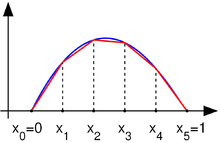
\includegraphics[scale=1.0]{fem.png}
    A function in  with zero values at the endpoints (blue), and a piecewise
    linear approximation (red)

\end{definition}

\begin{definition}[Odd function]\label{oddfunc}
    A function with the same values when you rotate 180 degrees around...
    \begin{align}
        - f(x) &= f(-x) \\
        f(x) + f(-x) &= 0
    \end{align}
    See also~\nameref{evenfunc}
\end{definition}

\begin{definition}[Even function]\label{evenfunc}
    Kind of like a mirror (90 degrees) around an axis;
    \begin{align}
        f(x) &= f(-x) \\
    \end{align}
    See also~\nameref{oddfunc}
\end{definition}

\begin{definition}[Pathological]
    Something that is counter-intuitive. The opposite is \textbf{well-behaved}.

\end{definition}

\begin{definition}[Parabola]
    A U-shaped, 2d, symmetrical curve.
\end{definition}

\begin{definition}[Parameterization]
    Represent a curve as a function.
    \begin{align}
        x = \cos{t} \\
        y = \sin{t}
    \end{align}
    is the parametric representation of a unit circle.

\begin{definition}[Partial derivative]
    Given a function $f$ with multiple parameters, a partial derivative is a
    derivative with respect to one of those variables.

    Partial derivatives are often denoted by $\partial$.

    To use partial derivation, you often assume that the other variables are 
    constants. Otherwise, there is an infinite number of tangent lines at
    any point, so you will have to have some range on the tangents.

\end{definition}

\end{definition}

\begin{definition}[Partial differential equation]
    A set of variables, and equations that show how they are all linked 
    together.
\end{definition}

\begin{definition}[Power series]\label{powerseries}
    \begin{align}
        f(x) = \sum\limits_{n=0}^{\infty}{a_{n}{(x-c)}^{n}}
    \end{align}
\end{definition}

\begin{definition}[Rectangle function]
    $$
    \Pi(x) = \left\{
            \begin{array}{l l}
                0 & \text{for} x > \frac{1}{2} \\
                \frac{1}{2} & \text{for} x = \frac{1}{2} \\
                1 & \text{for} x < \frac{1}{2} \\
            \end{array}
        \right.
    $$
\end{definition}

\begin{definition}[Reference value]
    The optimal/starting value. Note that when calculating differences,
    a reference value implies that order matters, i.e.\ $x - y \neq y - x$.

\end{definition}

\begin{definition}[Residual]
    In numerical analysis, this is the error from a result.
    E.g.\ in integration we have something-something + $C$, where C is the 
    the residual.

    It can (perhaps betterly) be stated that residuals is the error that occurs
    when approximating a function.

\end{definition}

\begin{definition}[Riemanns sum]\label{riemannsum}
    Sum from an integral. Divide the area under/over a curve into rectangles
    or trapezoids, and sum together their area. The smaller the shapes, the
    better.

    It is important to note that~\nameref{riemannsum} is an approximation - 
    one can not perfectly reconstruct the area under a curve.
\end{definition}

\begin{definition}[Risk function]
    Gives the expected value from a lossy function (compare two results, diff).
\end{definition}

\begin{definition}[Sine wave]
or sinusoid is a mathematical curve that describes a smooth repetitive
oscillation.

Its most basic form as a function of time $(t)$ is:

$y(t) = A\sin(2 \pi f t + \varphi) = A\sin(\omega t + \varphi)$
where:
\begin{description}
    \item[A], the amplitude, is the peak deviation of the function from zero.
    \item[f], the ordinary frequency, is the number of oscillations (cycles)
        that occur each second of time.
    \item[ω] = 2πf, the angular frequency, is the rate of change of the
    function argument in units of radians per second 
    \item[$\varphi$], the phase, specifies (in radians) where in its cycle the
        oscillation is at t = 0. I.e.\ the ``horizontal shift'' from a regular
        sine wave(????).
    If you e.g.\ represent two functions, $f(x) = \sin{x}$ and $g(x) = \sin{x} + 3$
    , the difference, i.e.\ phase shift, is 3. Note that these two functions
    have the same amplitude and frequency.
\end{description}

\end{definition}

\begin{definition}[Standard form]
    To write a number as a power of 10.
\end{definition}

\begin{definition}[Taylor series]
    A representation of a function as an infinite sum of terms that are 
    calculated from the derivatives at a point in the function.
    The formula is:
    \begin{align}
        \sum\limits_{n=0}^{\infty}{\frac{f^{(n)}(a)}{n!}{(x-a)}^{n}}
    \end{align}
\end{definition}

\begin{definition}[Shift invariant system]
    A discrete form of~\nameref{TIS} - the timesteps are discretized to follow
    a lattice spacing.
\end{definition}

\begin{definition}[Time invariant system]\label{TIS}
    A function with an output that does not depend on the output:
    \begin{align}
        x(t) &= y(t) \\
        x(t + \delta) &= y(t + \delta)
    \end{align}

    One example is the derivative function of polynomials (and others?) -
    no matter what timestep you choose - the value if the same.

    The ``antonym'' would be a time variant system.
\end{definition}

\begin{definition}[Translation invariant system]
    A system such that after a translation from A to T, any operator
    applied to A yields the same results in T.
\end{definition}

\begin{definition}[Unity]
    The number one. ``Unit functions'', ``unit circles'' all have the number 1.
\end{definition}

\begin{definition}[Univariate]
    An equation with only one variable.
\end{definition}

\begin{definition}[Vector Field]\label{vectorfield}
    An assigment of direction for a given set of points in an euclidian space.
    E.g.\ select every (10n, 10n) pixels in an image and get their derivative.
\end{definition}

\begin{definition}[Window function]
    A function that is zero outside of a given domain.
\end{definition}
